\chapter{soutions polarization}
\begin{abox}
	Practice set 1 solutions
	\end{abox}
\begin{enumerate}
\begin{minipage}{\textwidth}
	\item $\text { Consider three polarizer's } P_{1}, P_{2} \text { and } P_{3} \text { placed along an axis as shown in the figure. }$\\
	\begin{figure}[H]
		\centering
		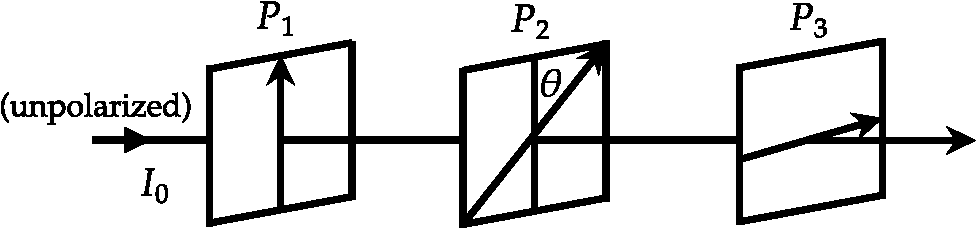
\includegraphics[height=3cm,width=9cm]{diagram-20211011(8)-crop}
	\end{figure}
	The pass axis of $P_{1}$ and $P_{3}$ are at right angles to each other while the pass axis of $P_{2}$ makes an angle $\theta$ with that of $P_{1}$. A beam of unpolarized light of intensity $I_{0}$ is incident on $P_{1}$ as shown. The intensity of light emerging from $P_{3}$ is
	\exyear{NET 2011}
\end{minipage}
\begin{tasks}(2)
	\task[\textbf{A.}]0
	\task[\textbf{B.}] $\frac{I_{0}}{2}$
	\task[\textbf{C.}]$\frac{I_{0}}{8} \sin ^{2} 2 \theta$
	\task[\textbf{D.}]$\frac{I_{0}}{4} \sin ^{2} 2 \theta$
\end{tasks}
\begin{answer}
	$I=I_{0} \cos ^{2} \theta$ (Malus Law)
	$$
	\Rightarrow I_{1}=\frac{I_{0}}{2}, \quad I_{2}=\frac{I_{0}}{2} \cos ^{2} \theta, \quad I_{3}=\frac{I_{0}}{2} \cos ^{2} \theta \times \cos ^{2}(90-\theta)=\frac{I_{0}}{8} \sin ^{2} 2 \theta \text {. }
	$$
	The correct option is \textbf{(c)}	
\end{answer}
\begin{minipage}{\textwidth}
	\item A beam of unpolarized light in a medium with dielectric constant $\in_{1}$ is reflected from a plane interface formed with another medium of dielectric constant $\in_{2}=3 \in_{1}$. The two media have identical magnetic permeability. If the angle of incidence is $60^{\circ}$, then the reflected light
	\exyear{NET 2015}
\end{minipage}
\begin{tasks}(1)
	\task[\textbf{A.}] is plane polarized perpendicular to the plane of incidence
	\task[\textbf{B.}] is plane polarized parallel to the plane of incidence
	\task[\textbf{C.}]is circularly polarized
	\task[\textbf{D.}] has the same polarization as the incident light
\end{tasks}
\begin{answer}
	\begin{figure}[H]
		\centering
		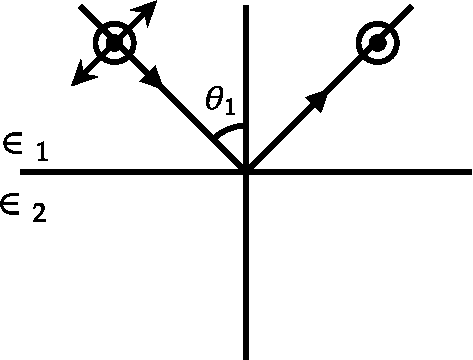
\includegraphics[height=4cm,width=6cm]{diagram-20211011(37)-crop}
	\end{figure}
	$$
	\begin{aligned}
	&\text { Solution: } \theta_{B}=\tan ^{-1}\left(\frac{n_{2}}{n_{1}}\right) \\
	&\theta_{B}=\tan ^{-1}\left(\frac{\sqrt{\epsilon_{2}}}{\sqrt{\epsilon_{1}}}\right)=\tan ^{-1}(\sqrt{3})
	\end{aligned}
	$$
	$\Rightarrow \theta_{B}=60^{\circ}$ (hence reflected light is plane polarized perpendicular to plane of incidence))\\
	The correct option is \textbf{(a)}	
\end{answer}
\begin{minipage}{\textwidth}
	\item The electric field of an electromagnetic wave is
	$$
	\vec{E}(z, t)=E_{0} \cos (k z+\omega t) \hat{i}+2 E_{0} \sin (k z+\omega t) \hat{j}
	$$
	where $\omega$ and $k$ are positive constants. This represents
	\exyear{NET 2016}
\end{minipage}
\begin{tasks}(1)
	\task[\textbf{A.}] a linearly polarised wave travelling in the positive $z$-direction
	\task[\textbf{B.}]a circularly polarised wave travelling in the negative $z$-direction
	\task[\textbf{C.}]an elliptically polarised wave travelling in the negative $z$-direction
	\task[\textbf{D.}] an unpolarised wave travelling in the positive $z$-direction
\end{tasks}
\begin{answer}
	Amplitude along $\hat{i}$ is $E_{0}$ and along $\hat{j}$ is $2 E_{0}$. So resultant wave is elliptically polarised	\\
	The correct option is \textbf{(c)}
\end{answer}
\end{enumerate}
\newpage
\begin{abox}
	Practice set 2 solutions
	\end{abox}
\begin{enumerate}
\begin{minipage}{\textwidth}
	\item A circularly polarized monochromatic plane wave is incident on a dielectric interface at Brewaster angle. Which one of the following statements is correct?
	\exyear{GATE 2013}
\end{minipage}
\begin{tasks}(1)
	\task[\textbf{A.}] The reflected light is plane polarized in the plane of incidence and the transmitted light is circularly polarized.
	\task[\textbf{B.}]The reflected light is plane polarized perpendicular to the plane of incidence and the transmitted light is plane polarized in the plane of incidence.
	\task[\textbf{C.}]The reflected light is plane polarized perpendicular to the plane of incidence and the transmitted light is elliptically polarized.
	\task[\textbf{D.}]There will be no reflected light and the transmitted light is circularly polarized.
\end{tasks}
\begin{answer}
	The correct option is \textbf{(c)}	
\end{answer}
\begin{minipage}{\textwidth}
	\item An unpolarized light wave is incident from air on a glass surface at the Brewster angle. The angle between the reflected and the refracted wave is
	\exyear{GATE 2014}
\end{minipage}
\begin{tasks}(2)
	\task[\textbf{A.}] $0^{\circ}$
	\task[\textbf{B.}]$45^{\circ}$
	\task[\textbf{C.}]$90^{\circ}$
	\task[\textbf{D.}]$120^{\circ}$
\end{tasks}
\begin{answer}
	The correct option is \textbf{(c)}	
\end{answer}
\begin{minipage}{\textwidth}
	\item A plane wave $(\hat{x}+i \hat{y}) E_{0} \exp [i(k z-\omega t)]$ after passing through an optical element emerges as $(\hat{x}-i \hat{y}) E_{0} \exp [i(k z-\omega t)]$, where $k$ and $\omega$ are the wavevector and the angular frequency, respectively. The optical element is a
	\exyear{GATE 2015}
\end{minipage}
\begin{tasks}(2)
	\task[\textbf{A.}] quarter wave plate
	\task[\textbf{B.}] half wave plate
	\task[\textbf{C.}] polarizer
	\task[\textbf{D.}]Faraday rotator
\end{tasks}
\begin{answer}
	Incident wave: $(\hat{x}+i \hat{y}) E_{0} e^{i \theta}=\left[E_{0} \cos \theta \hat{x}-E_{0} \sin \theta \hat{y}\right]$\\
	Left circular polarization with phase angle $\phi_{1}=-\theta=\theta e^{i \pi}$\\
	Emergent wave: $(\hat{x}-i \hat{y}) E_{0} e^{i \theta}=\left[E_{0} \cos \theta \hat{x}+E_{0} \sin \theta \hat{y}\right]$\\
	Right circular polarization with phase angle $\phi_{1}=+\theta=\theta e^{i 0}$\\
	Thus there is phase change of $\pi$ and hence path difference is $\frac{\lambda}{2}$.\\
	The correct option is \textbf{(b)}	
\end{answer}
\begin{minipage}{\textwidth}
	\item A quarter wave plate introduces a path difference of $\lambda / 4$ between the two components of polarization parallel and perpendicular to the optic axis. An electromagnetic wave with $\vec{E}=(\hat{x}+\hat{y}) E_{0} e^{i(k z-\omega t)}$ is incident normally on a quarter wave plate which has its optic axis making an angle $135^{\circ}$ with the $x$-axis as shown. The emergent electromagnetic wave would be
	\exyear{GATE 2018}
	\begin{figure}[H]
		\centering
		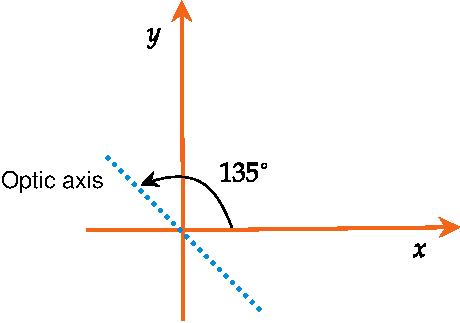
\includegraphics[height=4cm,width=6cm]{143-crop}
	\end{figure}
\end{minipage}
\begin{tasks}(1)
	\task[\textbf{A.}] elliptically polarized
	\task[\textbf{B.}]circularly polarized
	\task[\textbf{C.}]linearly polarized with polarization as that of incident wave
	\task[\textbf{D.}]linearly polarized but with polarization at $90^{\circ}$ to that of the incident wave
\end{tasks}
\begin{answer}
	The correct option is \textbf{(c)}	
\end{answer}

\begin{minipage}{\textwidth}
	\item The electric field of an electromagnetic wave is given by $\vec{E}=3 \sin (k z-\omega t) \hat{x}+$ $4 \cos (k z-\omega t) \hat{y}$. The wave is
	\exyear{GATE 2019}
\end{minipage}
\begin{tasks}(1)
	\task[\textbf{A.}] linearly polarized at an angle $\tan ^{-1}\left(\frac{4}{3}\right)$ from the $x$-axis
	\task[\textbf{B.}]linearly polarized at an angle $\tan ^{-1}\left(\frac{3}{4}\right)$ from the $x$-axis
	\task[\textbf{C.}] elliptically polarized in clockwise direction when seen travelling towards the observer
	\task[\textbf{D.}] elliptically polarized in counter-clockwise direction when seen travelling towards the observer
\end{tasks}
\begin{answer}
	At $z=0, E_{x}=-3 \sin \omega t, E_{y}=4 \cos \omega t$\\
	At $\omega t=0, E_{x}=0, E_{y}=4$\\
	$\text { At } \omega t=\frac{\pi}{2}, E_{x}=-3, E_{y}=0	$\\
	\begin{figure}[H]
		\centering
		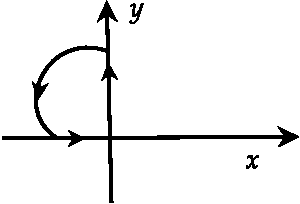
\includegraphics[height=3cm,width=5cm]{pic-crop}
	\end{figure}
	The correct option is \textbf{(d)}
\end{answer}
\begin{minipage}{\textwidth}
	\item In a set of $N$ successive polarizers, the $m^{\text {th }}$ polarizer makes an angle $\left(\frac{m \pi}{2 N}\right)$ with the vertical. A vertically polarized light beam of intensity $I_{0}$ is incident on two such sets with $N=N_{1}$ and $N=N_{2}$, where $N_{2}>N_{1} .$ Let the intensity of light beams coming out be $I\left(N_{1}\right)$ and $I\left(N_{2}\right)$, respectively. Which of the following statements is correct about the two outgoing beams?
	\exyear{GATE 2019}
\end{minipage}
\begin{tasks}(1)
	\task[\textbf{A.}] $I\left(N_{2}\right)>I\left(N_{1}\right) ;$ the polarization in each case is vertical
	\task[\textbf{B.}]$I\left(N_{2}\right)<I\left(N_{1}\right)$; the polarization in each case is vertical
	\task[\textbf{C.}]$I\left(N_{2}\right)>I\left(N_{1}\right)$; the polarization in each case is horizontal
	\task[\textbf{D.}]$I\left(N_{2}\right)<I\left(N_{1}\right)$; the polarization in each case is horizontal
\end{tasks}
\begin{answer}
	$$
	\begin{gathered}
	I\left(N_{1}\right)=I_{0}\left[\cos \left(\frac{n / 2}{N_{1}}\right)\right]^{2 N_{1}}, I\left(N_{2}\right)=I_{0}\left[\cos \left(\frac{n / 2}{N_{2}}\right)\right]^{2 N_{2}} \\
	I\left(N_{2}\right)>I\left(N_{1}\right)
	\end{gathered}
	$$
	For last polarization, pass axis will be horizontal.
	$\mathrm{Ex}: N_{1}=5$
	$$
	\begin{aligned}
	&I(5)=I_{0}\left[\cos \left(18^{*}\right)\right]^{10}=0.605 I_{0} \\
	&N_{2}=10 \\
	&I(10)=I_{0}\left[\cos \left(9^{*}\right)\right]^{20}=0.780 I_{0} \\
	&I(10)>I(5)
	\end{aligned}
	$$
	The correct option is \textbf{(c)}	
\end{answer}
\begin{minipage}{\textwidth}
	\item When unpolarised light is incident on a glass plate at a particular angle, it is observed that the reflected beam is linearly polarized. What is the angle of the refracted beam with respect to the surface normal?
	\exyear{JEST 2012}
\end{minipage}
\begin{tasks}(1)
	\task[\textbf{A.}] $56.7^{0}$
	\task[\textbf{B.}]$33.4^{0}$
	\task[\textbf{C.}]$23.3^{0}$
	\task[\textbf{D.}]The light is completely reflected and there is no refracted beam.
\end{tasks}
\begin{answer}
	Since $n_{1}=1, n_{2}=1.52$\\
	Brewster angle $\theta_{B}=\tan ^{-1}\left(\frac{n_{2}}{n_{1}}\right)=\tan ^{-1}\left(\frac{1.52}{1}\right)=56.7^{0}$\\
	Now $\theta_{R}=180-90-56.7=33.4^{0}$\\
	The correct option is \textbf{(b)}	
\end{answer}
\begin{minipage}{\textwidth}
	\item $\text { The electric field } \vec{E}=E_{0} \sin (\omega t-k z) \hat{x}+2 E_{0} \sin \left(\omega t-k z+\frac{\pi}{2}\right) \hat{y} \text { represents: }$
	\exyear{JEST 2016}
\end{minipage}
\begin{tasks}(1)
	\task[\textbf{A.}] a linearly polarized wave
	\task[\textbf{B.}]a right-hand circularly polarized wave
	\task[\textbf{C.}]a left-hand circularly polarized wave
	\task[\textbf{D.}]an elliptically polarized wave
\end{tasks}
\begin{answer}
	The correct option is \textbf{(d)}
\end{answer}
\end{enumerate}